\section{Discussion of results}
\subsection{Initial results}
Early in the project an experiment was conducted to determine which model to keep working with. The choice was between the four models in \autoref{imagenet} where the modified U-Net model initialized with ImageNet weights showed the lowest validation loss after 150 epochs, and because of this the model was chosen to see if the performance could be further improved by augmentation.

\subsection{Augmentation results}
Our expectation would be the model performance would increase if the model would be trained on augmented data. However, as seen in \autoref{augres} training on augmented data makes the modified U-Net model perform worse, and in some cases a lot worse. In some cases this seem to stem from over augmentation, as when we compare the results of training on the original, large rotation and large shearing data compared to training on the original, small rotations and small shearing data. Simply making smaller rotations and smaller shearing gives us significantly better results. Over augmentation is likely also the reason the mix model perform worse. For the model trained on the original and arc data, the arcing effect might alter the image too much resulting in the model learning suboptimal features. Because CNN's are translation and rotation invariant it would be expected that the original and horizontal model and the original and large rotations model would perform as good as simply training on the original dataset, however, this is not the case. Although both of these models achieve a good validation loss it is still worse than the validation loss of the model trained on the original training set. This would indicate that substituting augmented data into the training set makes the model overfit relatively more than it does on the original data alone. As we remove some data to add the augmented data this points in the direction of our model not having enough data to train on or at least it only have a few images with some quite important features which seems to be replaced by less important features after augmentation. This second idea seem to be strengthened by \autoref{concat} where although triple the amount of data is used to train the model, the validation loss does not improve which would indeed indicate the augmented data does not 'catch' the 'rare' features of the original dataset and thus does not increase the variety of data but instead adds more of the same 'kind' of data.\\
One could have conducted experiments by increasing or decreasing the number original images in the training sets to see if this would influence the assumed overfitting in the models trained on augmented data. An experiment have however been conducted to see the importance of image sizes, however the results are inconclusive and can be seen in the appendix.

\subsection{Test results}

\begin{wrapfigure}[25]{l}{0.3\linewidth}
	\vspace{-1.5cm}
	\centering
	\vspace{1cm}
	\begin{subfigure}[b]{\linewidth}
		\centering
		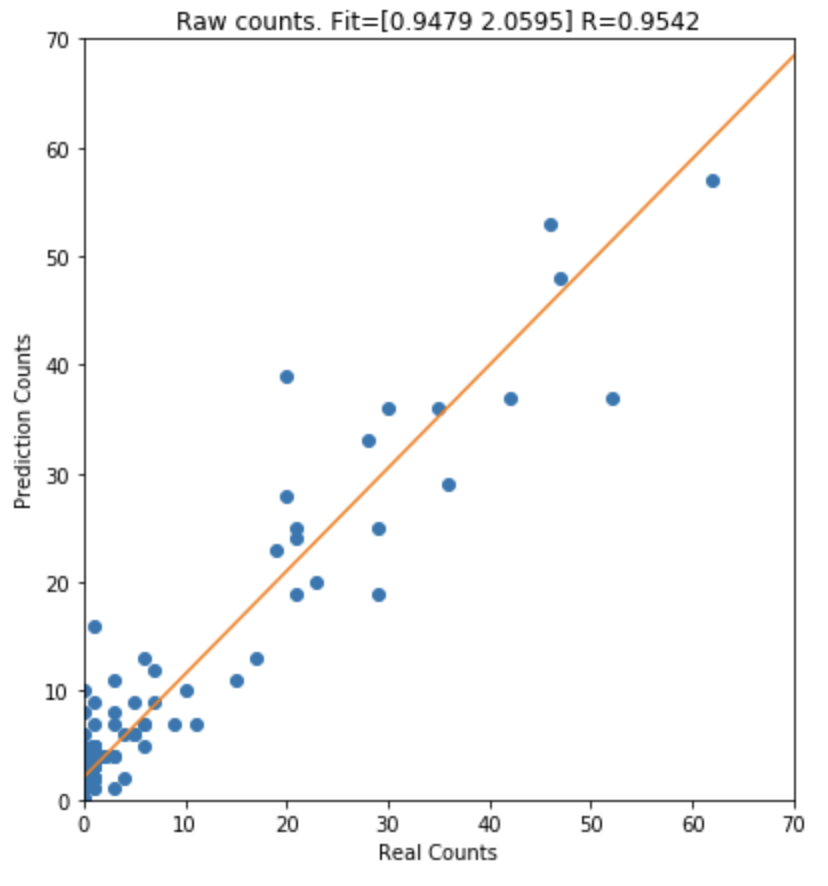
\includegraphics[width=\linewidth]{Materials/Results/Test/OriginalLine}
		\caption{Results for the model trained on the original dataset.\newline}
	\end{subfigure}
	\\
	\begin{subfigure}[b]{\linewidth}
		\centering
		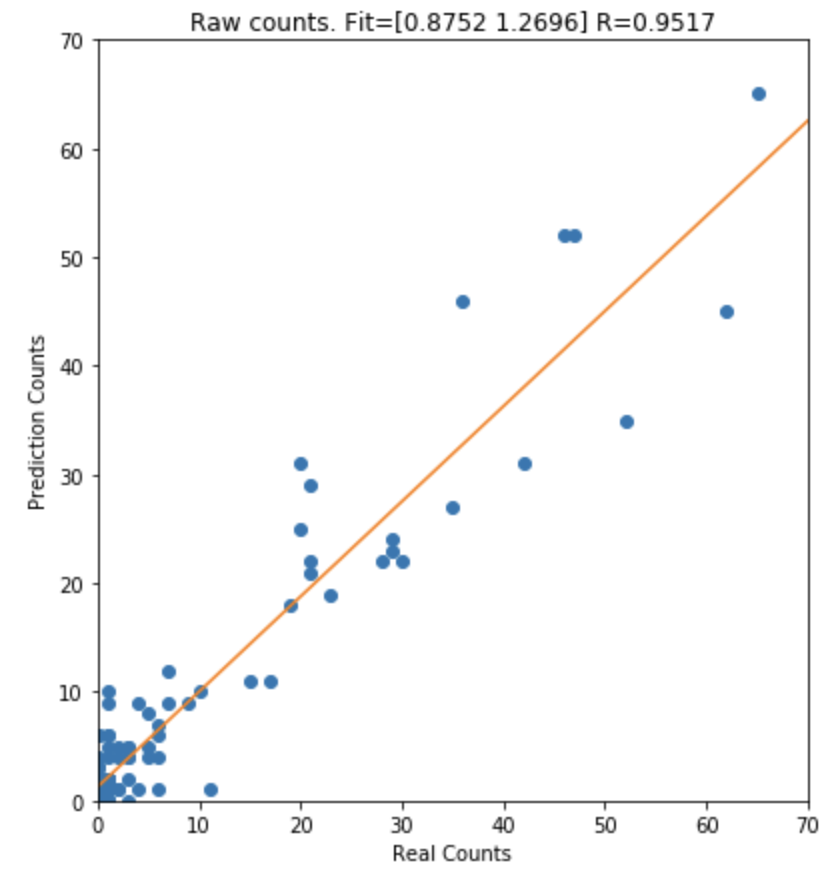
\includegraphics[width=\linewidth]{Materials/Results/Test/AugLine}
		\caption{Results for the model trained on the original, small rotations and small shearing dataset.}
	\end{subfigure}
	\caption{Results of the circle count metric. A regression line has been fitted and plotted to show how close the results are to lie on a line with slope 1.}
	\label{circlecount}
\end{wrapfigure}

From \autoref{tableDice} we note when we remove all the results which gives a DICE of 0 the average DICE increases relatively more for the model trained on augmented data than the model trained on the original data. Getting an increase in DICE when removing zero results means the predictions made are closer to the true mask as predicting too many or too few dots results in a lower DICE which would lower the average. This relative increase in DICE equalizes between the models as we increase the 'time intervals'. This might be due to the model trained on original data performs better on later time intervals than the model trained on augmented data or that predicting too many or too few dots becomes relatively less impactful the more dots that are present. This indicates the model trained on augmented data performs better on data with only a few dots than the model trained on the original data does. In \autoref{circlecount} we see this trend again as the model trained on the original data seemingly over predicts a lot of circles / puncta in images with a true count below 15 which the other model does not. However, we also see the model trained on the original data seem to predict the number of circles more accurately on images with a true count of more than 30 circles, whereas the model trained on augmented data seem to either over predict or under predict quite symmetrically.

\subsection{Automatic tool}
One goal of this project was to explore the possibility of automatic segmentation of two-photon microscopy images. Based on the results in \autoref{onesfivessixes} it seems this is not quite possible as the best models developed achieve an average DICE around 0.4. However, this does not mean these models can not be used when working with two-photon microscopy images. One could use the models to initially find some of the dots. Depending on if it is easier to find the dots or verify that a dot is placed correctly, this might save significant time. Based on the results in \autoref{circlecount} one can get an initial count of the circles in the images significantly faster than having to count manually. Although this might introduce some uncertainty, if one is only interested in an indication about the number of circles this might speed up work significantly.